% =============================================================================
% 5.4 语义桥接四档消融
% 草稿版本：v0.2 (2026-05-07)
%   v0.1：作为 5.2.3 子小节起草。
%   v0.2：按导师意见 3 提级为 5.4 \subsection，标题去掉前缀"通路 B"。
% 字数：约 1300 字
% 风格规则：v0.2 风格（无 \textbf / \textit / 引例括号 / 双引号 / 破折号）
% 引用：\cite{ref10, ref20}
% 图表：
%   - 图 \reffig{fig:bridge-ablation}       4 档分组柱状图（核心 4 指标）
%   - 表 \reftab{tab:bridge-by-category}    按要素类别拆分（71 条）
%   - 表 \reftab{tab:bridge-llm-trap}       LLM baseline 双指标对比
% 复用 4.1 节已有图表：\reftab{tab:bridge-ablation}（4 档总表）
% 依赖宏包：booktabs / tabularx / graphicx（主稿已加载）
% =============================================================================

\subsection{语义桥接四档消融}
\label{sec:bridge-eval}

通路 B 语义桥接的 4 档消融总表已在 \ref{sec:semantic-bridge} 节
\reftab{tab:bridge-ablation} 给出，对应核心 4 指标的可视化对照见
\reffig{fig:bridge-ablation}：\texttt{rule\_\bk{}plus\_\bk{}rag} 档在
覆盖率、\texttt{grade\_\bk{}id} 准确率、\texttt{must\_\bk{}cite} 全中与
\texttt{citation} 真实性四项核心指标上同时达到 100\%，
\texttt{llm\_\bk{}baseline} 档则在 \texttt{grade\_\bk{}id} 与
\texttt{must\_\bk{}cite} 两项关键合规指标上分别仅有 5.6\% 与 25.4\%。
本节聚焦三件 \ref{sec:semantic-bridge} 节未展开的内容：评测集设计与按
要素类别的差异化表现、大语言模型基线的真实却错幻觉模式归类，以及
与知识库标准核对表预演错误的呼应关系。

\begin{figure}[!ht]
    \centering
    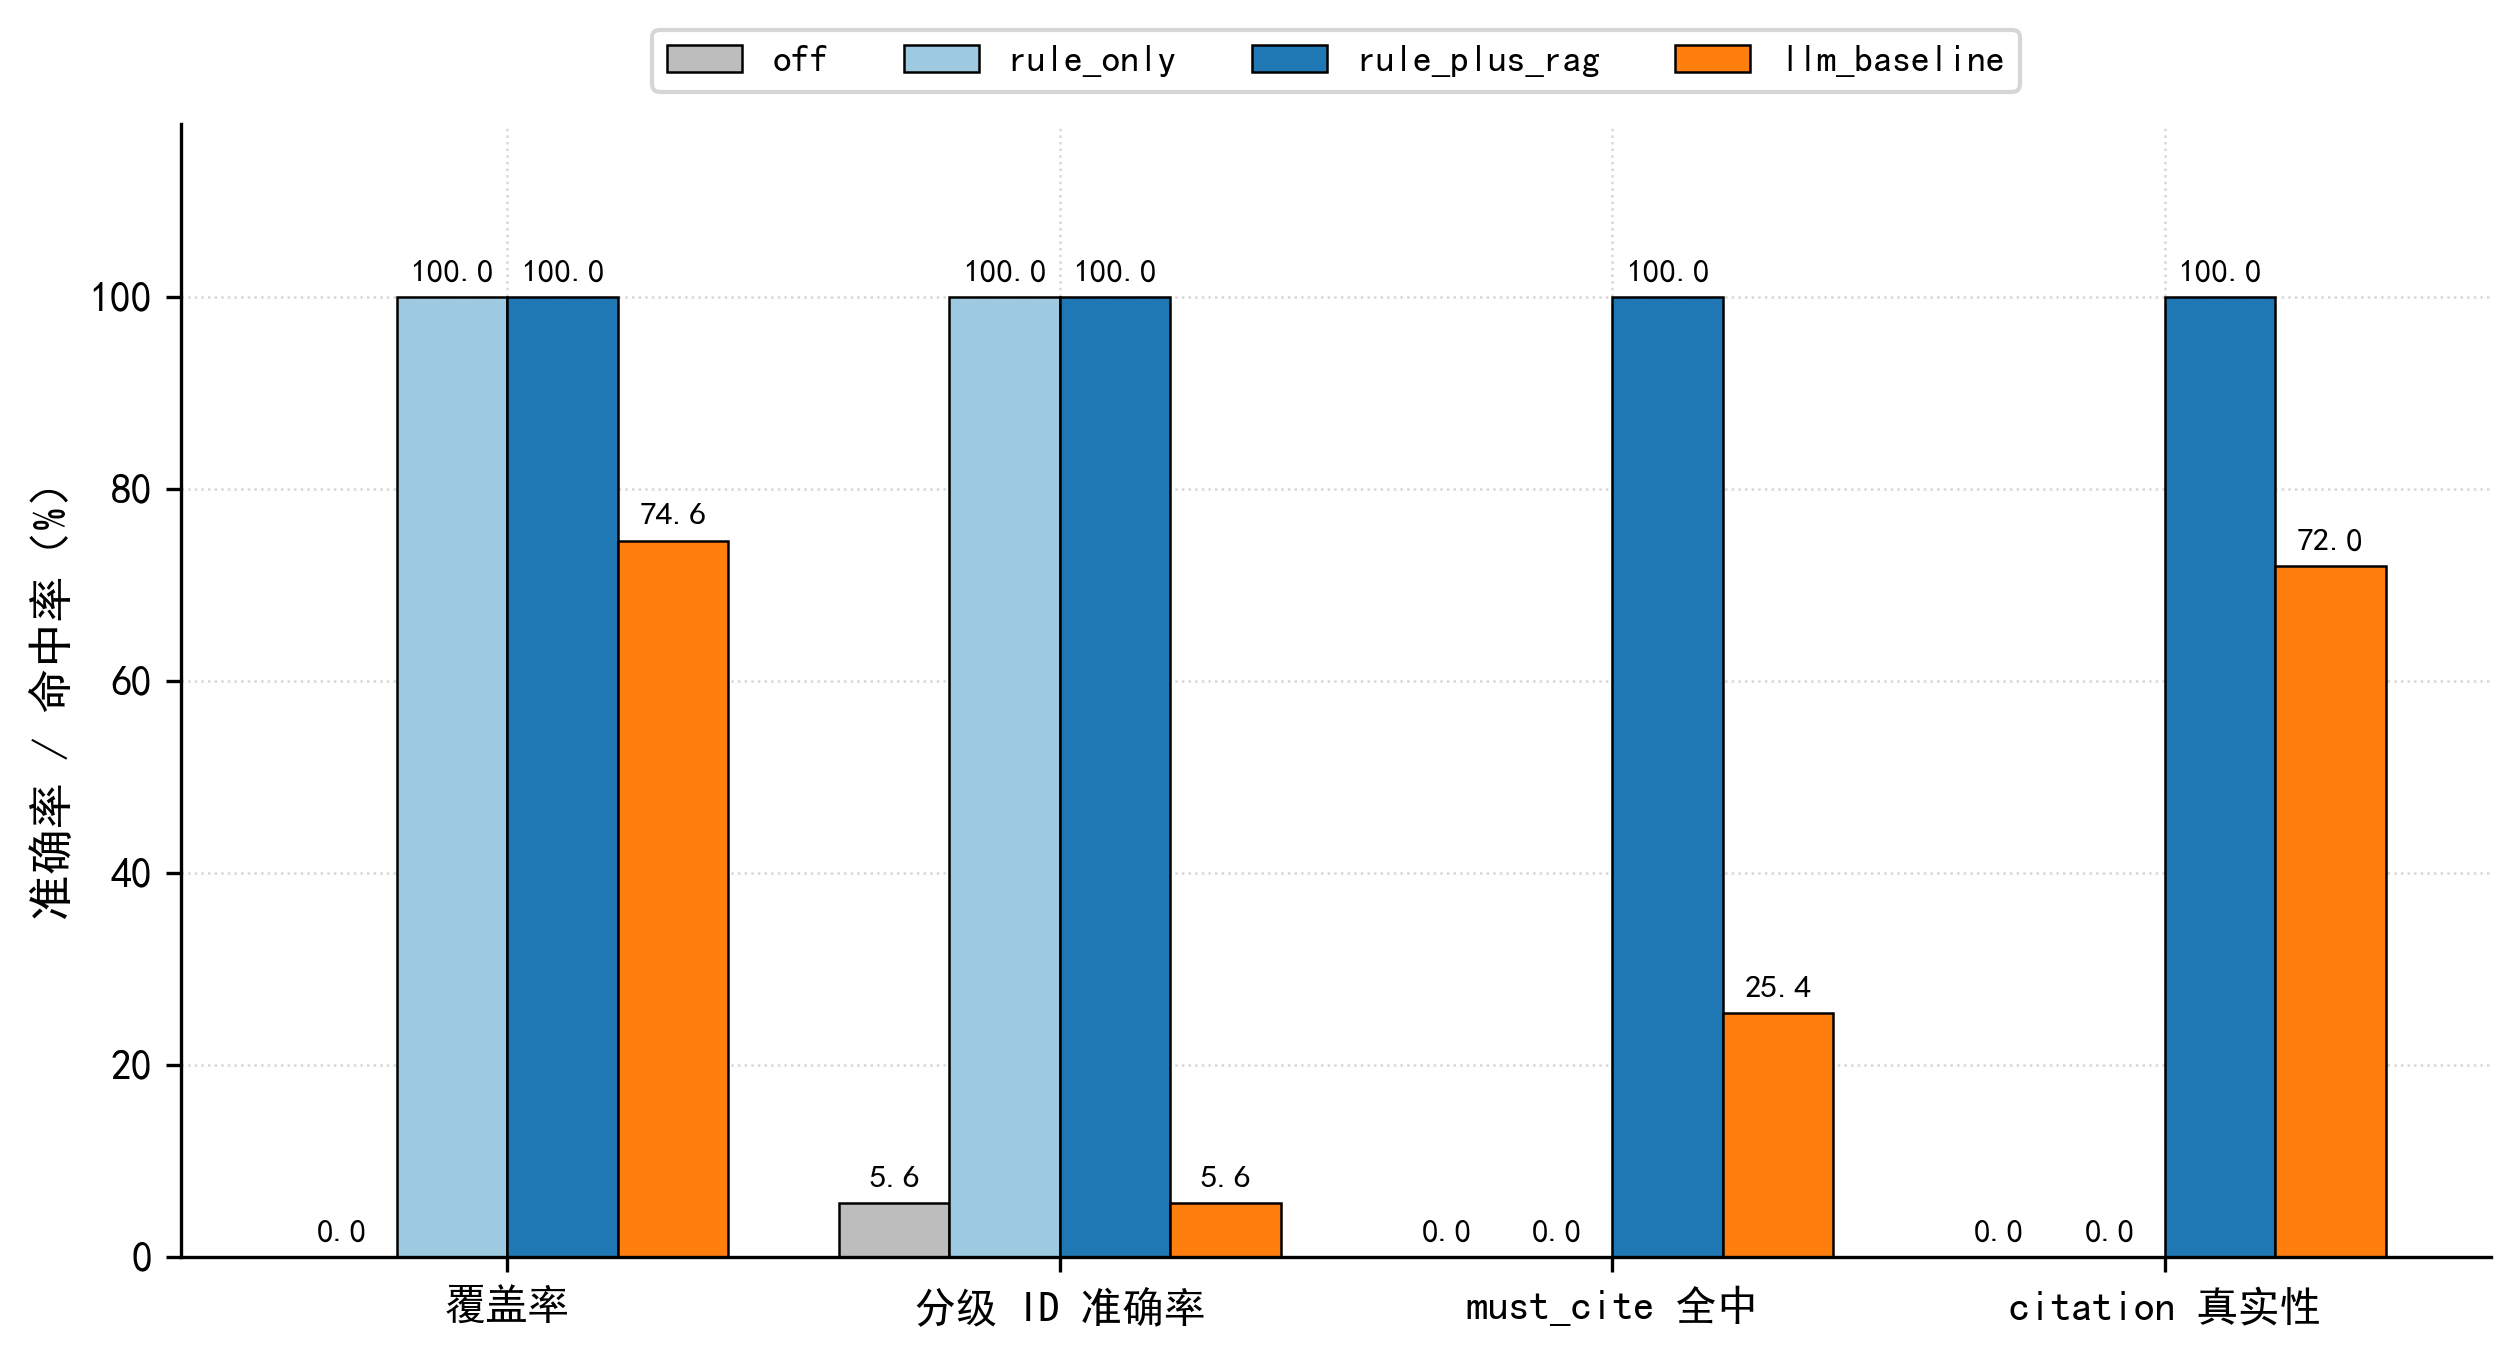
\includegraphics[width=0.92\linewidth]{figures/eval_5_2_bridge_ablation}
    \caption{通路 B 语义桥接四档消融核心指标对比}
    \label{fig:bridge-ablation}
\end{figure}

评测集为 \texttt{semantic\_\bk{}bridge\_\bk{}bench.\bk{}jsonl} 共 71 条用例，覆盖
9 类气象要素：24 小时降水、12 小时降水、风速、温度、能见度、湿度、
场景过滤负例、跨要素复合与 fallback 异常输入。每条用例标注期望输出的
\texttt{labels} 数组，每条标签包含 \texttt{grade}、\texttt{grade\_\bk{}id}、
\texttt{must\_\bk{}cite} 关键字、\texttt{source.\bk{}org}、\texttt{source.\bk{}doc\_\bk{}title}
五个字段。评测脚本 \texttt{experiments/\bk{}eval/\bk{}run\_\bk{}bridge\_\bk{}eval.\bk{}py} 在
4 档处理方式上分别跑 71 条用例：\texttt{off} 关闭桥接、\texttt{rule\_\bk{}only}
仅启用确定性分级器、\texttt{rule\_\bk{}plus\_\bk{}rag} 在分级基础上启用 RAG 富化、
\texttt{llm\_\bk{}baseline} 让大语言模型在不调任何工具的条件下从同一份输入
直接输出 \texttt{SemanticLabel} 列表，构成自由发挥的对照。

按要素类别拆分的结果见 \reftab{tab:bridge-by-category}。
\texttt{rule\_\bk{}only} 与 \texttt{rule\_\bk{}plus\_\bk{}rag} 两档在所有要素类别上的
\texttt{grade\_\bk{}id} 准确率均为 100\%。\texttt{llm\_\bk{}baseline} 档在
9 类要素的 \texttt{grade\_\bk{}id} 准确率几乎全部为 0\%，唯一的 100\% 来自
fallback 类的 4 条用例：这 4 条要求模型在面对非法或无关字段时输出空
\texttt{labels}，模型恰好正确判断而被记为通过，与生成质量无关。

\begin{table}[H]
    \centering
    \caption{通路 B 语义桥接按要素类别拆分}
    \label{tab:bridge-by-category}
    \song\fontsize{9pt}{12pt}\selectfont
    \renewcommand{\arraystretch}{0.95}
    \begin{tabular}{lrcccc}
        \toprule
        要素类别 & 用例数 & rule\_only · grade\_id & rule\_plus\_rag · cite & llm\_baseline · grade\_id & llm · cite 真实 \\
        \midrule
        24 h 降水 & 11 & 100\% & 100\% & 0\% & 100\% \\
        12 h 降水 & 5 & 100\% & 100\% & 0\% & 100\% \\
        风速 & 16 & 100\% & 100\% & 0\% & 100\% \\
        场景过滤负例 & 2 & 100\% & 100\% & 0\% & 100\% \\
        跨要素复合 & 2 & 100\% & 100\% & 0\% & 100\% \\
        fallback 异常 & 4 & 100\% & 100\% & 100\% & --- \\
        \bottomrule
    \end{tabular}
\end{table}

大语言模型基线的最具论证价值的发现是真实却错的双指标差距。具体数据
见 \reftab{tab:bridge-llm-trap}。\texttt{llm\_\bk{}baseline} 档给出的
\texttt{citation} 字段出现率为 100\%，且其中所引用的标准号粗粒度真实性
也是 100\%。换言之，模型给出的 GB/T 编号都是真实存在的国标。但是当
评测严格比较模型给的标准号加条款号是否与知识库期望一致时，命中率
跌到 25.4\%，57.6 个百分点的差距正是大语言模型 \texttt{citation}
幻觉的核心特征：模型知道有哪些标准存在，但不知道该用哪一个、哪一条。

\begin{table}[H]
    \centering
    \caption{大语言模型基线的真实却错双指标}
    \label{tab:bridge-llm-trap}
    \song\wuhao
    \begin{tabular}{lc}
        \toprule
        指标 & llm\_baseline 档数值 \\
        \midrule
        \texttt{citation} 出现率 & 100.0\% \\
        \texttt{citation} 标准号粗粒度真实性 & 100.0\% \\
        \texttt{must\_\bk{}cite} 关键字严格命中率 & 25.4\% \\
        \texttt{source.\bk{}doc\_\bk{}title} 字段精确匹配率 & 0.0\% \\
        场景过滤负例通过率 & 50.0\% \\
        \texttt{grade\_\bk{}id} 准确率 & 5.6\% \\
        \bottomrule
    \end{tabular}
\end{table}

逐条分析模型基线的失败用例可归纳出五类幻觉模式。第一类是标准号对、
条款号错。例如 4 条需要引用 JGJ 80-2016 的高空作业用例，模型分别
给出了 §5.1.3、§5.1.6、§3.0.3、§3.0.5 四个不同条款号，全部错误，正确
条款号是 §3.0.8。这是典型的模式记忆型幻觉，模型记住了 JGJ 80 的条款
大致是 §3.0.X 或 §5.1.X 形式，便在合理样式空间中随机生成。第二类是
自创等级与越界处理失败。例如把 12 小时降水 100 mm 标为 12 小时大暴雨，
但 GB/T 28592-2012 的 12 小时表只到暴雨即 $\geq 30\,\mathrm{mm}$，
没有 12 小时大暴雨档；把蒲福 15 级风混入 GB/T 19201-2006 热带气旋等级，
混用了两个独立标准。第三类是分级名误名，例如把蒲福 5 级清劲风 fresh
breeze 写为清风，与国标条文用词不严格相符。第四类是 \texttt{grade\_\bk{}id}
凭印象编造。模型给出的 ID 形如 \texttt{heavy\_\bk{}rain} 或 \texttt{beaufort\_\bk{}5}，
而知识库的真实 ID 为 \texttt{grading\_\bk{}precip\_\bk{}24h\_\bk{}heavy} 或
\texttt{grading\_\bk{}wind\_\bk{}beaufort\_\bk{}5}，36 条非 fallback 用例没有一条与
知识库命名约定一致。第五类是场景过滤失败。\texttt{rule\_\bk{}plus\_\bk{}rag}
通过 \texttt{applicable\_\bk{}scene} 元数据在场景不匹配时主动不输出
\texttt{citation}，模型基线在所有场景下都倾向于输出 \texttt{citation}
而无法分辨该说与不该说，场景过滤负例通过率仅 50\%。

这五类幻觉与本文知识库人工核对环节预先发现的错误模式存在惊人的呼应
关系。知识库 1.0 版本中本就存在 JGJ 80-2016 §3.0.4 与真实 §3.0.8 的
错位、寒潮误引 GB/T 20484、蒲福 0 级 $<0.3\,\mathrm{m/s}$ 与真实
$0.0\sim0.2\,\mathrm{m/s}$ 的微误等问题，这些问题被人工核对修正后
仍然在大语言模型基线中以同样的模式重新出现。这印证了一条独立判断：
人工核对中暴露的错误模式不是知识库构建者的低级失误，而是大语言模型
在涉及精确编号引用任务上的内在偏差 \cite{ref20}，仅依靠模型自身能力
无法消除 \cite{ref10}。这构成了一个自洽的论证闭环：人工核对发现典型
错误，模型基线复现同样错误，桥接架构通过 \texttt{grade\_\bk{}id} 硬链接
加场景元数据避免错误。
